% tADRguide.tex
% v1.0 released January 2013

\documentclass{tADR2e}

% The following packages can be found on http:\\www.ctan.org
\usepackage{caption}
\usepackage{color}
\usepackage{graphicx} % for pdf, bitmapped graphics files
%\usepackage{epsfig} % for postscript graphics files
\usepackage{mathptmx} % assumes new font selection scheme installed
%\usepackage{times} % assumes new font selection scheme installed
\usepackage{amsmath} % assumes amsmath package installed
\usepackage{amssymb}  % assumes amsmath package installed
\usepackage{mathrsfs}
\DeclareMathOperator*{\argmin}{argmin}
\usepackage{algorithm}
\usepackage{algpseudocode}  %\usepackage[noend]{algpseudocode}
\algtext*{EndWhile}% Remove "end while" text
\algtext*{EndIf}% Remove "end if" text
\usepackage{booktabs}
\usepackage{multirow}
\usepackage{proof}
\newtheorem{property}{Property}
\usepackage[numbers]{natbib}

\makeatletter
%\let\NAT@parse\undefined % allow hyperref to work with ieeeconf.cls for bib numbers
\makeatother
\usepackage{hyperref}
%\usepackage{cite}


% Math shortcuts :
\newcommand\real{\mathbb{R}}
\newcommand\p{\mathbf{p}}
\newcommand\pii{\mathbf{p_{i,i+1}}}
\newcommand\pij{\mathbf{p_{i,j}}}
\newcommand\gT{\tilde{g}^T}
\newcommand\g{\tilde{g}}
\newcommand\CS{\mathcal{C}}
\newcommand\dimCS{n_\mathbf{C}}
\newcommand\body{{\cal B}}
\newcommand\Sone{\mathbf{S}^1}
\newcommand\Sthree{\mathbf{S}^3}
\newcommand\conf{\mathbf{q}}
\newcommand\xx{\mathbf{x}}
\newcommand\cost{C}
\newcommand\weight{W}
\newcommand\translation{\mathbf{t}}
\newcommand\tcolli{t_{coll\ i}}


%%%%%%%%%%%%%%%%%%%%%%%%%%%%%%%%%%%%%%%%%%%%%%%%%%%%%%%%%%%%%%%%%%%%%%%%%%%%%%%%
\begin{document}
\graphicspath{{images/}}

\jvol{00} \jnum{00} \jyear{2013} \jmonth{January}

\articletype{GUIDE}

\title{{\itshape Advanced Robotics} A simple path optimization method for motion planning }	

\author{Myl\`{e}ne Campana$^{a,b}$ $^{\ast}$ \thanks{$^\ast$Corresponding author. Email: mcampana@laas.fr}, Florent Lamiraux$^{a,b}$ and Jean-Paul Laumond$^{a,b}$
\\\vspace{6pt}
$^{a}${\em{LAAS-CNRS, Toulouse, France}};
$^{b}${\em{ This work has been supported by the project ERC Advanced Grant 340050 Actanthrope and by the FP~7 project Factory in a Day under grant agreement n°~609206 }}
}
\maketitle

\begin{abstract}
Most algorithms in probabilistic sampling-based path planning compute 
collision-free paths made of straight line segments lying in the configuration 
space. Due
to the randomness of sampling, the paths make detours that need to be optimized.
The contribution of this paper is to propose a gradient-based algorithm that
transforms a polygonal collision-free path into a shorter one, while both:
\begin{itemize}
\item requiring mainly collision checking, and few time-consuming obstacle 
distance computation,
\item constraining only part of the configuration variables that may cause a 
collision, and not the entire configurations, and
\item reducing parasite motions that are not useful for the problem resolution.
\end{itemize}
The algorithm is simple and requires few parameter tuning. Experimental
results include navigation and manipulation tasks, e.g. an robotic arm 
manipulating throw a window and a PR2 robot working in a kitchen environment, 
and comparisons with a random shortcut optimizer.

\medskip

\begin{keywords}path optimization; motion planning; robotics
\end{keywords}\medskip

\end{abstract}


\section{Introduction}

Motion planning for systems in cluttered environments has been addressed for more
than thirty years~\citep{ref-motionplan},~\citep{ref-pianomover}. Most planners
today randomly sample the system configuration space~\cite{ref-spaceconfig} in
order to find a collision-free path. The main issue using these techniques is
 that the computed path makes unnecessary detours and needs to be post-processed 
 before being executed by a virtual or real robot. Alternative
strategies exist however.
\begin{itemize}
\item Planning by path-optimization~\cite{itomp2012},~\cite{voronoiOMP} where
obstacle avoidance is handled by constraints or cost using computation of the
nearest obstacle distance. Most of these planners are using non-linear
optimization~\cite{BettsNonlinopt} under constraints.
   
Such planners provide close-to-optimality paths and have smaller time computation
for easy problems, but they are mostly unable to solve narrow passage issues.
 
\item Optimal random sampling~\cite{KaramanPRMstarRRTstar} are also close to an
optimal solution, but computation time is significantly higher than classical
approaches. Moreover the roadmap is only valid for a given motion planning
   problem. 
\end{itemize}

In this paper, we propose a method aimed at shortening path length after a path
planning step. Note that we do not address path planning, but that we take the
result of a probabilistic motion planner as the input to our path optimization 
method.

For this shortening purpose, random shortcut methods are
still very popular~\cite{Sekhavat-Svestka1998,HauserFastSmooth}. However, random 
shortcut requires fine tuning of the termination condition (see 
Algorithm~\ref{algo:random-shortcut}) and is no efficient due to randomness for long trajectories where only a small part needs to be optimized. Figure~\ref{decoupled_DOF_optimization} presents another situation where random shortcut will always fail to optimize the initial path, since it cannot decouple the robot degrees of freedom (DOF) on which the optimization occurs, contrary to our algorithm.

\begin{figure}[H]
	\centering
	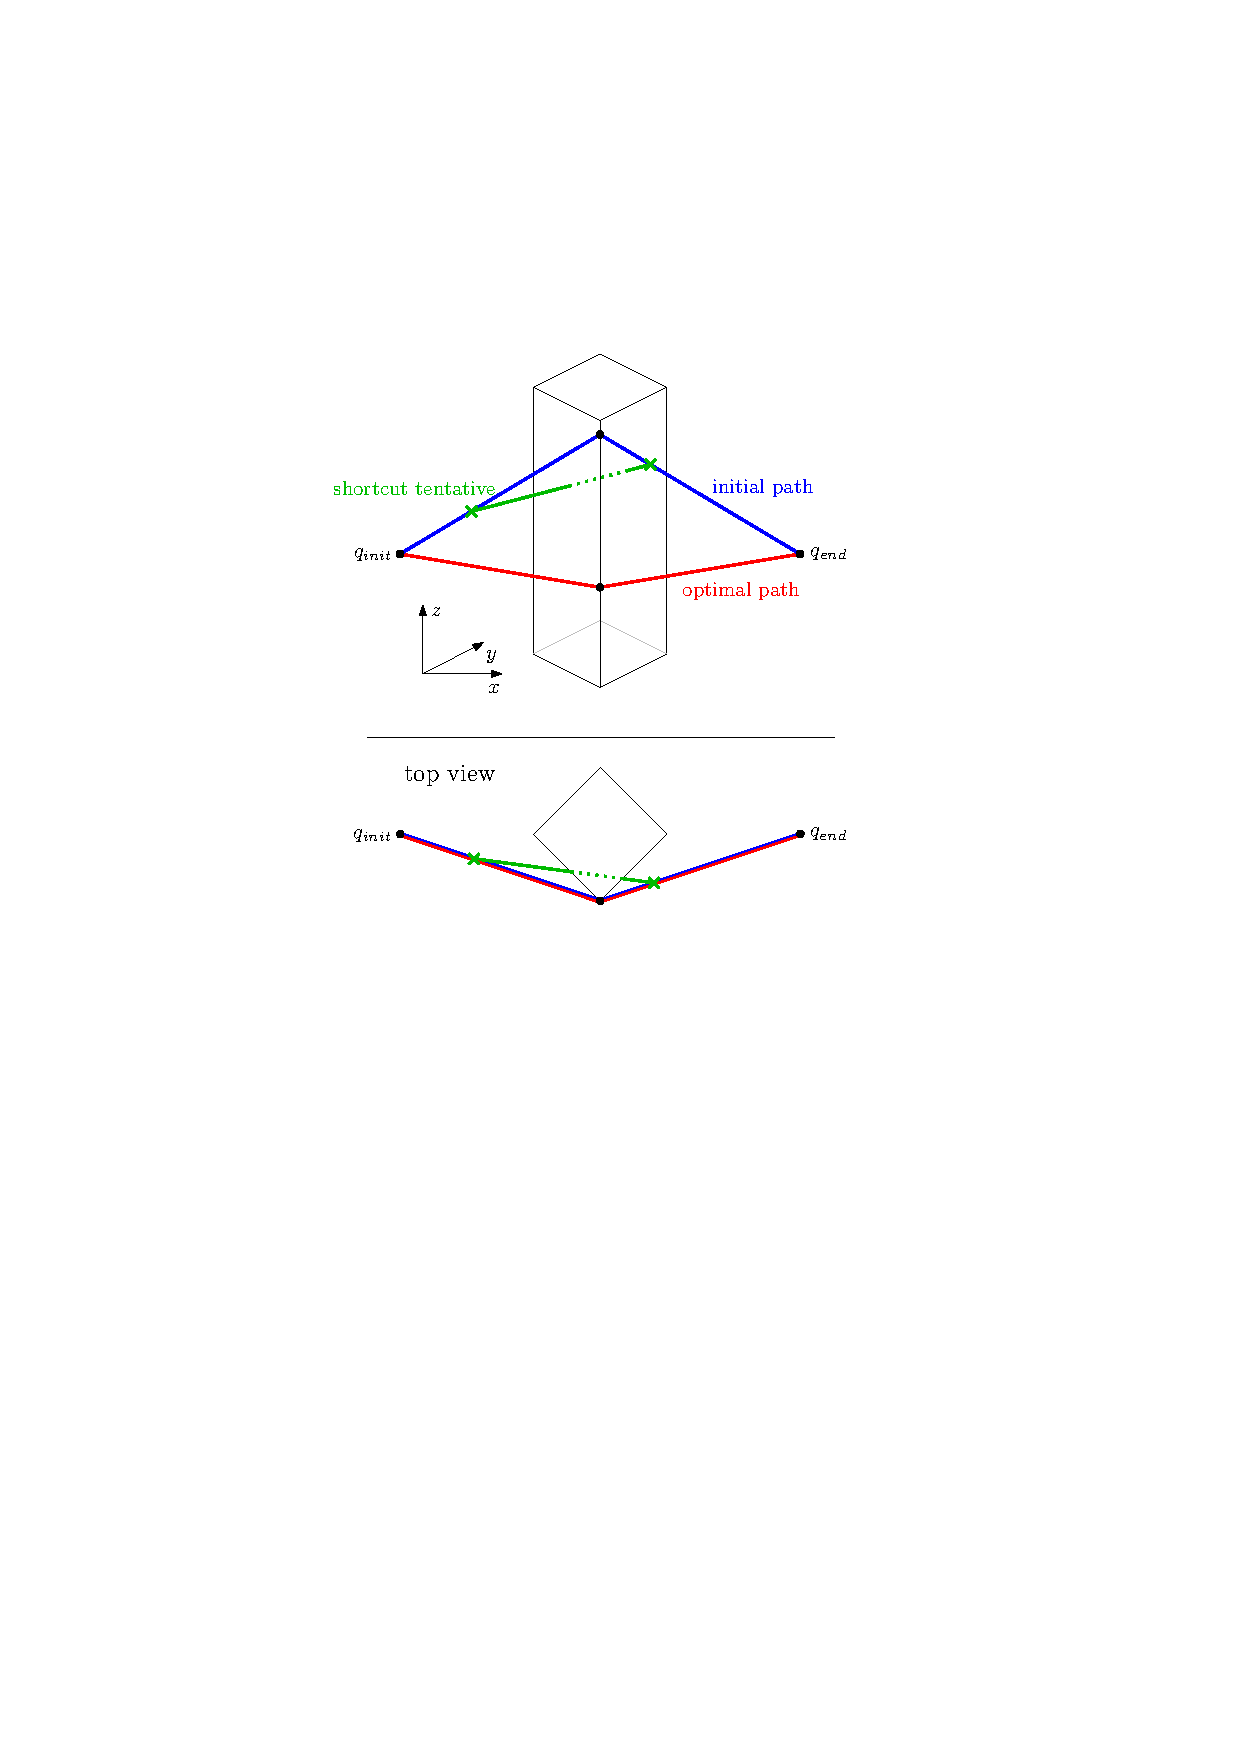
\includegraphics[width=7.5cm]{decoupled_DOF_optimization.pdf}
	\caption{Example of a path which random shortcut will never manage to 
	optimize: each shortcut tentative will provide a collision or will not 
	decrease the path length. The optimal path belongs to the $x-y$ plane 
	containing $q_{init}$ and $q_{end}$.}
	\label{decoupled_DOF_optimization}
\end{figure}


On the other hand, numerical
optimization methods like CHOMP~\cite{RatliffChomp} can be used as a
post-processing step. They have clear termination conditions, but collision
avoidance is handled by inequality constraints sampled at many points along
the trajectory. These methods therefore require a pre-processing step of the
robot (and/or environment) model in order to make 
it simpler:~\cite{RatliffChomp} covers PR2 bodies with spheres, 
while~\cite{convexOptimMotplan} needs to decompose objects into convex subsets.
Moreover, in the applications we address, optimality is not desirable as
such since the shortest path between two configurations in a cluttered
environment usually contains contacts with the obstacle,
or is most of the time
out of the scope of numerical optimization algorithms~\cite{LaumondOptim}.

The idea of our method is to find a good trade-off between
the simplicity of “blind” methods like shortcut algorithm,
and the complexity of distance based optimization techniques.
The method iteratively shortens the initial path with gradient-based information.
When a collision is detected at a given iteration, the method backtracks to the
latest valid iteration and inserts a linearized transformation constraint
between the objects detected in collision. Only few distances between objects are evaluated, therefore no pre-processing of the
robot or environment models is necessary. The underlying optimization
algorithm is a quadratic program.

Related work is presented in Section II. Section III explains how the 
path-optimizer works, from the formulation of the problem to the implemented
algorithm. Finally, we conclude on experimental results in Section IV.




\section{RELATED WORK}

CHOMP algorithm~\cite{RatliffChomp} optimizes an initial guess provided as
input. It minimizes a time invariant cost function using efficient covariant
hamiltonian gradient descent. The cost is quantified by non-smooth parts (with
high velocities) and an obstacle avoidance term, provided by the distance to the 
nearest obstacle for each iteration of the trajectory. Calculating these nearest 
distances however is time-consuming because the distances between all pairs of 
objects must be computed at each time step along the path. To reduce the 
computation time, the method starts by building offline a map of distances that 
will be called during the optimization at the requested time. Besides, meshes 
are pre-processed into bounding spheres so that distances are computed faster 
at the cost of a geometry approximation.

STOMP method~\cite{KalakrishnanStomp} avoids to compute an 
explicit gradient for cost optimization using a stochastic analysis of local 
random samples. But as for CHOMP, the obstacle cost term requires a voxel map to 
perform its Euclidian Distance Transforms, and represents the robot bodies with 
overlapping spheres. Such technique provides lots of distance and penetration 
information but remains very time consuming and is not as precise as some 
distance computation techniques based on the problem meshes as 
Gilbert-Johnson-Keerthi~\cite{gilbertGjk}.

Some optimization-based planners may not require an initial guess but some naive 
straight-line manually or randomly-sampled initialization as 
TrajOp~\cite{SchulmanConvexOptim}. Its trajectory is iteratively optimized with 
sequential convex optimization by minimizing at each step its square length, 
linear and non-linear constraints considered as penalties. To compute the 
collision-constraints, nearest obstacle distances are calculated at each discrete 
time of the trajectory vector. This can be a burden for a high-dimensional robot 
or a complex environment as we propose to use, and may be compensated with a 
short path composed of only one or two waypoints.


The elastic strips framework~\cite{BrockElasticStrips} is also an optimization 
based method. The path is modeled as a spring and obstacles give rise to a 
repulsive potential field. Although designed for on-line control purposes, this 
method may be used for path shortening. In this case however, the number of 
distance computation is very high. The authors also proposed to approximate the 
robot geometry by spheres.

Some heuristics use random shortcuts on the initial guess combined with a 
trajectory re-building that returns ${C}^1$ shortcuts made of parabolas and lines 
(bang-bang control)~\cite{HauserFastSmooth}. These local refined trajectories 
are time-optimal since they comply with acceleration and velocity constraints. 

In some way, our method shares similarities with~\cite{PanSmoothSplineShort} 
since this latter method relies on collision checking and backtracks when an 
iteration is detected in collision, instead of trying to constantly satisfy 
distance constraints. Unlike our method however, the iterations are composed of 
Cubic-B-splines. The benefit of this method is that the result is a 
differentiable path.

TO DESCRIBE:

~\cite{Guernane2011} (guiding shoots) is ``locally optimal'', not addressing high-DOF problems, 

~\cite{Geraerts04clearancebased}, whereas just implemented for freeflyer robots, is using medial axis retractation for clearance and a partial random shortcut (applied only on random DOF) which can address the problem of ~\ref{decoupled_DOF_optimization} but has longer computation time and is not using the information returned by the checker of which links are colliding to guide the shortcut.


\section{PATH OPTIMIZATION} \label{section:path_optim}

\subsection {Kinematic chain}

A robot is defined by a kinematic chain composed of a tree of joints. We denote 
by $(J_1,\cdots,J_m)$ the ordered list of joints. Each joint $J_i$, $1\leq i\leq 
m$ is represented by a mapping from a sub-manifold of $\real^{n_i}$, where $n_i$ 
is the dimension of $J_i$ in the configuration space, to the space 
of rigid-body motions $SE(3)$. The rigid-body motion is the position of the joint 
in the frame of its parent. In the examples shown in this paper, we consider 4 
types of joints described in Table~\ref{tab:joints}.
\begin{table}[b]
\centerline {
  \begin{tabular}{cccc}
    Name & dimension & config space & velocity\\
    \hline
    translation & 1 & $\real$ & $\real$\\
    bounded rotation & 1& $\real$ & $\real$\\
    unbounded rotation & 2 & $\Sone\subset\real^2$ & $\real$\\
    $SO(3)$ & 4 & $\Sthree\subset\real^4$ & $\real^3$
  \end{tabular}
}
\caption {Translation and rotation joint position are defined by 1 
parameter corresponding respectively to the translation along an axis and a 
rotation angle around an axis. Unbounded rotation is defined by a point on the 
unit circle of the plane: 2 parameters corresponding to the cosine and the 
sine of the rotation angle. $SO(3)$ is defined by a unit quaternion. The 
velocity of translation and unbounded rotation joints is the derivative of the 
configuration variable. The velocity of an unbounded rotation joint corresponds 
to the angular velocity. The velocity of a $SO(3)$ joint is defined by the 
angular velocity vector $\omega\in\real^3$.}
\label{tab:joints}
\end{table}
A configuration of the robot
$$\conf = (\underbrace{q_1,\cdots,q_{n_1}}_{J_1},\underbrace{q_{n_1+1},
\cdots,q_{n_1+n_2}}_{J_2},\cdots q_n),\ n\triangleq\sum_{i=1}^m n_i$$
is defined by the concatenation of the joint configurations. The configuration 
space of the robot is denoted by $\CS\subset\real^n$.

Note that the configuration of the robot belongs to a sub-manifold of $\real^n$.

The velocity of each joint $J_i$, $1\leq i \leq m$ is defined by a vector of $
\real^{p_i}$, where $p_i$ is the number of DOF of $J_i$. Note that 
the velocity vector does not necessarily have the same dimension as the 
configuration vector.

The velocity of the robot is defined as the concatenation of the velocities of 
each joint.
$$\dot{\conf} = (\underbrace{\dot{q}_{1},\cdots,\dot{q}_{p_1}}_{J_1},
\underbrace{\dot{q}_{p_1+1},\cdots,\dot{q}_{p_1+p_2}}_{J_2},\cdots \dot{q}_p),\ p
\triangleq\sum_{i=1}^m p_i$$

\paragraph {Operations on configurations and vectors} by analogy with the case 
where the configuration space is a vector space, we define the following 
operators between configurations and vectors:
$$
\conf_2 - \conf_1 \in \real^p, \ \conf_1, \conf_2\in\CS
$$
is the constant velocity moving from $\conf_1$ to $\conf_2$ in unit time, and
$$
\conf + \dot{\conf}\in\CS, \ \conf\in\CS \ \dot{\conf}\in\real^p
$$
is the configuration reached from $\conf$ after following constant velocity $
\dot{\conf}$ during unit time.

Note that the definitions above stem from the Riemanian structure of the 
configuration space of the robot. The above sum corresponds to the exponential 
map. We do not have enough space in this paper to develop the theory in a more 
rigorous way. The reader can easily state that ``following a 
constant velocity'' makes sense for the four types of joints defined in 
Table~\ref{tab:joints}. We refer to~\cite{riemanian-optim2008} Chapter~5 for 
details about Riemanian geometry.

\subsection {Straight interpolation}

Let $\conf_1, \conf_2\in\CS$ be two configurations. We define the straight 
interpolation between $\conf_1$ and $\conf_2$ as the curve in $\CS$ defined on 
interval $[0,1]$ by:
$$
t \rightarrow \conf_1 + t (\conf_2 - \conf_1)
$$
This interpolation corresponds to the linear interpolation for translation and 
bounded rotations, to the shortest arc on $\Sone$ for unbounded rotation and to 
the so called slerp interpolation for $SO(3)$.

\subsection{Problem definition}

We consider as input a path composed of a concatenation of straight 
interpolations between $wp+2$ configurations: $(\conf_0, \conf_1,\cdots,\conf_{wp
+1})$. This path is the output of a random sampling path planning algorithm 
between $\conf_0$ and $\conf_{wp+1}$. We wish to find a sequence of waypoints $
\conf_{1}$,...,$\conf_{wp}$ such that the new path $(\conf_0, \conf_1,\cdots,
\conf_{wp+1})$ is shorter and collision-free. Note that $\conf_0$ and $\conf_{wp
+1}$ are unchanged and that the workspace of the robot contains obstacles. We 
denote by $\xx$ the optimization variable:
$$
\xx \triangleq (\conf_1,\cdots,\conf_{wp})
$$

\subsubsection {Cost}

let $W\in\real^{p\times p}$ be a diagonal matrix of weights:
$$
W=\left(\begin{array}{cccccccccc}
w_1 I_{p_1}       &        &  0  \\
    & w_2 I_{p_2} &        &   \\
    &            & \ddots &   \\
  0 &            &        & w_m I_{p_m}
\end{array}\right)
$$
where $I_{p_i}$ is the identity matrix of size $p_i$ and $w_i$ is the weight 
associated to joint $J_i$. We define the length of the straight interpolation 
between two configurations as:
$$
\|\conf_2 - \conf_1\|_{W} \triangleq \sqrt{(\conf_2 - \conf_1)^T W^2 (\conf_2 - 
\conf_1)}.
$$
Weights are used to homogenize translations and rotations in the velocity vector. 
For rotations, the weight is equal to the maximal distance of the robot bodies 
moved by the joint to the center of the joint.

Given $\conf_0$ and $\conf_{wp+1}$ fixed, the cost we want to minimize is defined 
by
$$
\cost (\xx) \triangleq \frac{1}{2}\sum_{i=1}^{wp+1} \lambda_{i-1} \|\conf_{i}-\conf_{i-1}\|_{W}
^{2}
$$
where the $\lambda_{i-1}$ coefficients benefit will be explained in the results 
section. For now we can assume that $\forall i,\, \lambda_{i-1}=1$.

Note that $\cost$ is not exactly the length of the path, but it can be 
established that minimal length paths also minimize $\cost$. This latter cost is 
better conditioned for optimization purposes.

\subsection {Resolution}
We assume that the direct interpolation between the initial and final configurations contains collisions.
Let $H$ denotes the constant Hessian of the cost function, an iteration is 
described as follow:
\begin{equation}\label{eq:iteration-1}
\begin{split}
& \pii =  -H^{-1} \nabla c(\xx_i)^{T} \\
& \xx_{i+1} =  \xx_{i} + \alpha_i \pii
\end{split} 
\end{equation}
where $\alpha_i$ is a real valued parameter. Taking $\alpha_i=1$ yields the 
unconstrained minimal cost path, i.e. all waypoints aligned on the straight line 
between $q_0$ and $q_{n+1}$. Since this solution is in collision, we set 
$\alpha_i = \alpha$ 
where $\alpha$ is a parameter that will be explained in the algorithm section.

We iterate step~(\ref{eq:iteration-1}) until path $\xx_{i+1}$ is in collision. 
When a collision is detected, we introduce a constraint and perform a new 
iteration from $\xx_i$ as explained in the next section. We use a continuous 
collision checker inspired of~\cite{SchwarzerExactCollision} to validate our 
paths and to return the first colliding configuration along a path. This step corresponds to \texttt{validatePath} in Algorithm~\ref{algo:gradient}.

\subsection{Constraints}

\begin{figure}[b]
	\centering
	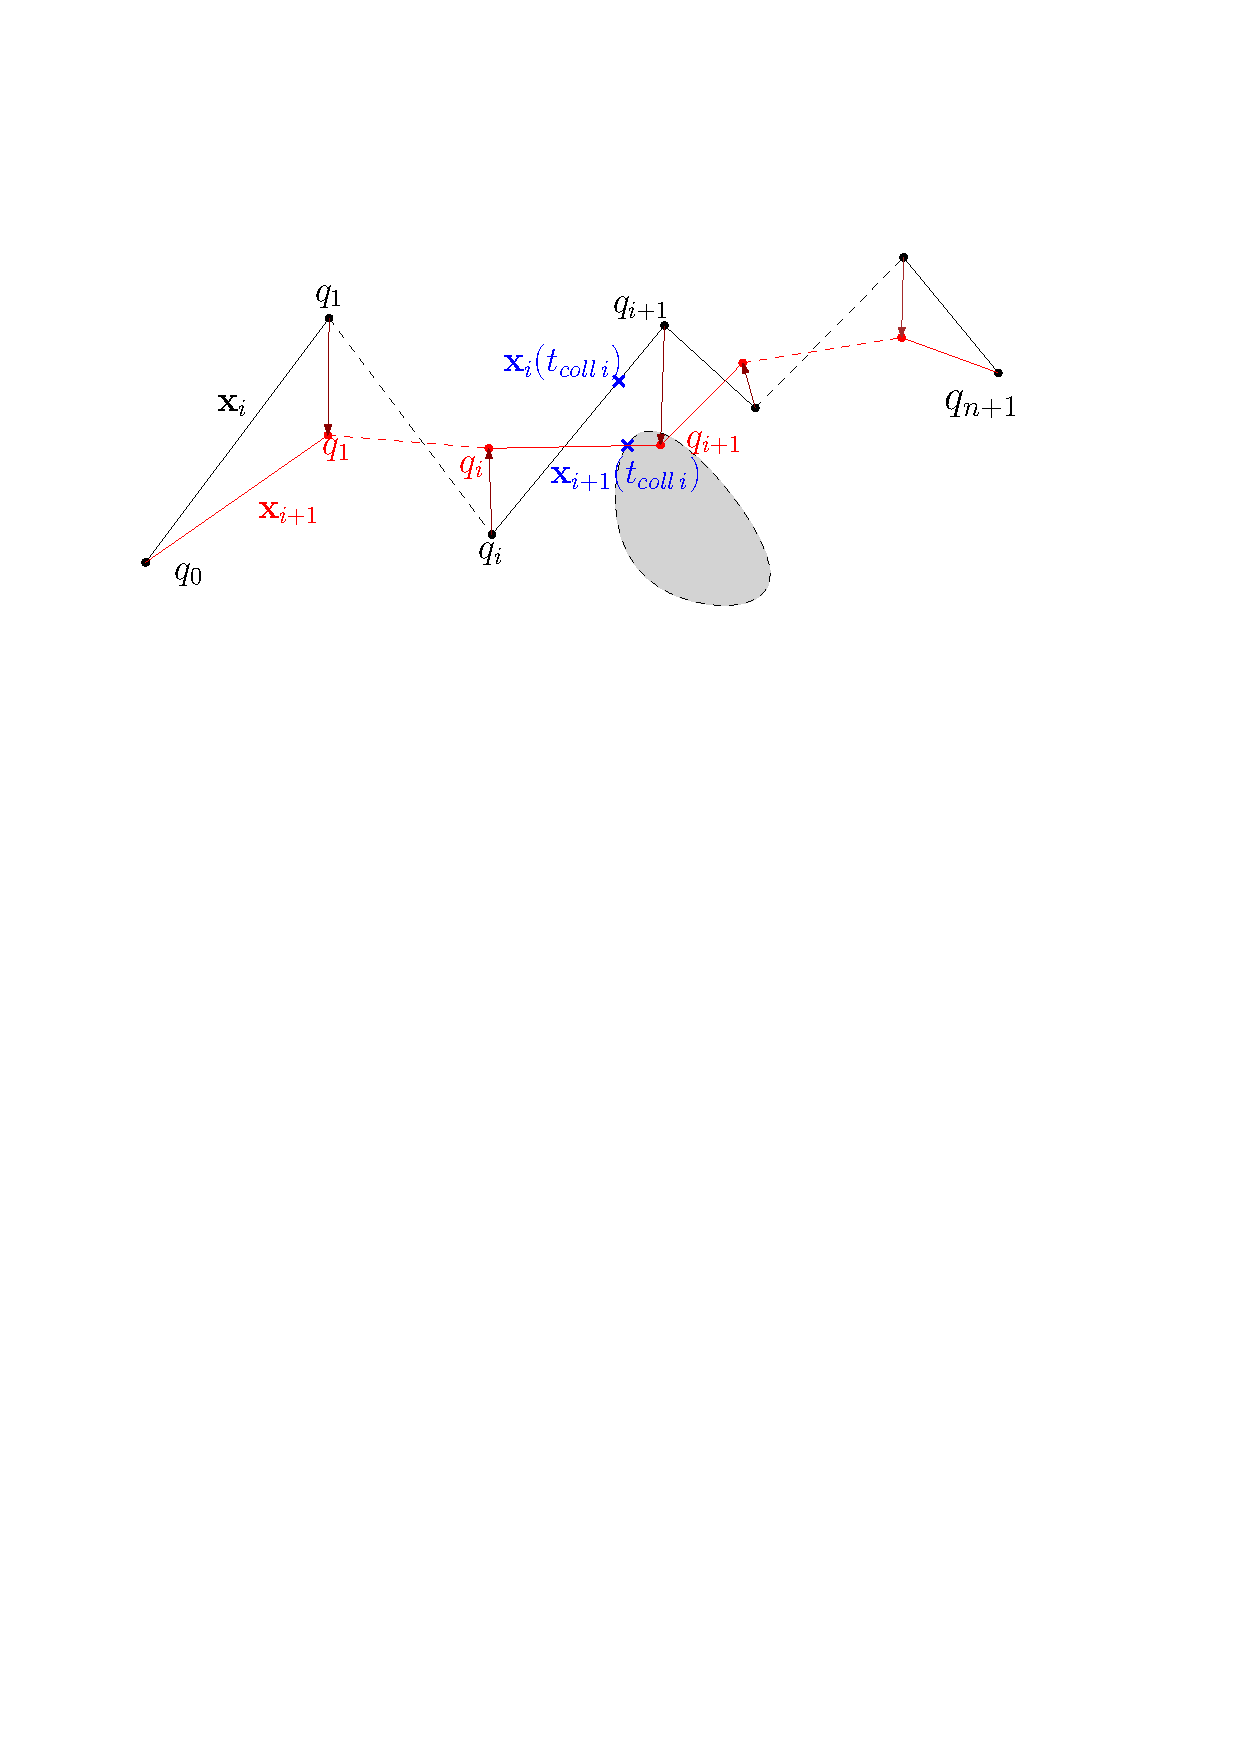
\includegraphics[width=8cm]{optim_grad.pdf}
	\caption{Illustration of one iteration of our optimization. $\xx_{i+1}$ 
	appears 
	to be in collision with the obstacle, the first colliding configuration 
	$\xx_{i+1}(\tcolli)$ is returned by the continuous collision checker. The corresponding constraint will be computed in configuration $\xx_{i}(\tcolli)$.}
	\label{optim_grad}
\end{figure}

Let $T$ be a positive real number such that each path $\xx_i$ is a mapping from 
interval $[0,T]$ into $\CS$: $\xx_i(0) = q_0$, $\xx_i(T) = q_{n+1}$ for all $i$. Let 
us denote by $\tcolli$ the abscissa of the first collision detected on path 
$\xx_{i+1}$, which previous iteration $\xx_i$ was collision-free (see 
Figure~\ref{optim_grad}). Thus in 
configuration $\xx_{i+1}(\tcolli)$ a collision has been 
detected. Two cases are possible:
\begin{enumerate}
\item the collision occurred between two bodies of the robot: $\body_1$ and $
\body_2$, or
\item the collision occurred between a body of the robot $\body_1$ and the 
environment.
\end{enumerate}
In the rest of this section, we will only consider the first case. Reasoning about the second case is similar, except that the 
constraint is on the transformation of $\body_1$ with respect to the environment.

\begin {figure}
  \centerline {
    \def\svgwidth {\linewidth}
    \graphicspath {{./images/}}
    \input {images/transformation-constraint.pdf_tex}
  }
  \caption {Transformation constraint notations.}
  \label{fig:transformation-constraint}
\end {figure}
Let $M^{*}\in SE(3)$ denote the homogeneous transformation between frames of $\body_1$  and $\body_2$ in configuration $\xx_i(\tcolli)$. Let $M\in SE(3)$ denote the same transformation in configuration $\xx (\tcolli)$ where $\xx$ is any path in $\CS^{wp}$. Let $R\in SO(3)$ (resp. $R^{*}$) and $\translation\in\real^3$ (resp. $\translation^{*}$) be the rotation and translation parts of $M$ (resp. $M^{*}$).
See also Figure~\ref{fig:transformation-constraint} for notations.

We denote by $F$ the mapping from $\CS^{wp}$ to $\real^6$ defined by
\begin{equation}\label{eq:constraint}
F (\xx) = \left(\begin{array}{c} R^T (\translation^{*} - \translation) \\
  \log (R^T R^{*})\end{array}\right)
\end{equation}
$\log (R^T R^{*})$ represents here a vector $\mathbf{v}$ of $\real^3$ such that
$R^T R^{*}$ is the rotation of axis $\mathbf{v}$ and of angle $\|\mathbf{v}\|$.
Note that $F$ vanishes for any path $\xx$ such that in configuration
$\xx(\tcolli)$ the relative position of $\body_2$ w.r.t. $\body_1$ is equal to $M^{*}$.
Let $r$ denotes the \textit{radius} of the bounding sphere of $\body_2$ centered at the origin of $\body_2$ local frame. Let us denote by $d$ the minimal distance between $\body_1$ and $\body_2$
in configuration $\xx_i(\tcolli)$. We have the following property.
\begin {property} \label {prop:collision free}
Let $\xx\in\CS^{wp}$ be a path and let us denote by $\translation$ and $\mathbf{v}$ respectively the 3 first coordinates and the 3 last coordinates of $F(\xx)$. If
$$
\|\translation\| + r \|\mathbf{v}\| \leq d
$$
then in configuration $\xx(\tcolli)$, $\body_1$ and $\body_2$ are collision-free.
\end {property}
The proof is straightforward: expressed in reference frame of $\body_1$, the motion of $\body_2$ between configurations $\xx(\tcolli)$ and $\xx_i(\tcolli)$ is a translation of vector $\translation$ followed by a rotation of angle $\|\mathbf{v}\|$. No point of $\body_2$ has moved by more than $\|\translation\| + r \|\mathbf{v}\|$. Therefore no collision is possible.

When a collision is detected at $\tcolli$ along path $\xx_{i+1}$, we wish to add
constraint
\begin{equation}\label{eq:non-linear constraint}
F (\xx) = 0
\end{equation}
However, as this constraint is non-linear, we linearize it around $\xx_i$:
$$
\frac{\partial F}{\partial \xx}(\xx_i)(\xx -\xx_i) = 0
$$
for any later iteration $\xx_j$, $j\geq i+1$.

We refer to~\cite{nocedal2006numerical} for solving constrained quadratic 
programs (QP). This corresponds to \texttt{computeIterate} in Algorithm~\ref{algo:gradient}.


\subsection{Algorithm}

In this part we describe the path-optimizer Algorithm~\ref{algo:gradient} 
according to the previous step definitions. The main difficulty here is to handle 
the scalar parameter $\alpha$ determining how much of the computed step $\p$ will 
be traveled through, and also to return a collision-free path. Typically, we 
chose $\alpha_{init} = 0.2$ to process small steps. $\alpha_{init} = 0.5$ is more 
encountered in the optimization literature, procuring larger steps but with more 
risks of collision.

\begin{algorithm}
\begin{algorithmic}%[1] % line numerotation
\Procedure{Optimize}{$\xx_0$}
	\State $\alpha \gets \alpha_{init}$
	\State $minReached \gets false$
	\While{($\textbf{not}(noCollision \textbf{ and } minReached)$)}
		\State $\p = \texttt{computeIterate}()$
		\State $minReached = (||\p||<10^{-3} \textbf{ or } \alpha=1)$
		\State $\xx_1 \gets \xx_0 + \alpha\,\p$
		\If{(\textbf{not}(\texttt{validatePath($\xx_1$)}))}
			\State $noCollision \gets false$
			\If{$(\alpha \neq 1)$}
				\State \texttt{addCollisionConstraints}()
				\State $\alpha \gets 1$
			\Else
				\State $\alpha \gets \alpha_{init}$
			\EndIf
		\Else
			\State $\xx_0 \gets \xx_1$
			\State $noCollision \gets true$
		\EndIf
	\EndWhile
	\Return $\xx_0$
\EndProcedure
\end{algorithmic}
\caption{Gradient-based path-optimization.} \label{algo:gradient}
\end{algorithm}

Each time a collision-constraint is added, 
the solution of the current QP is tested (i.e. $\alpha = 1$). If this path is collision-free, the algorithm returns it as the solution. Otherwise, 
smaller steps are iteratively applied and tested toward the minimum, and constraints are added each time a collision is found.


\section{RESULTS}

This part gathers optimization results performed on the planning software 
Humanoid Path Planner~\cite{hpp}. The initial trajectory is obtained with two 
kind of probabilistic planners: Visibility-PRM~\cite{visibility-prm} and 
RRT-connect~\cite{rrt-connect}.

\subsection{From 2D basic examples...}

\begin{figure}[t]
	\centering
	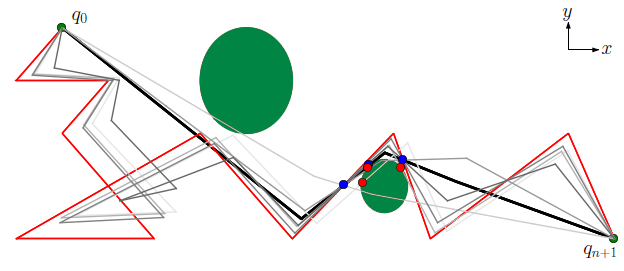
\includegraphics[width=7.5cm]{2d_final_green.png}
	%\noindent\rule{8cm}{0.8pt}
	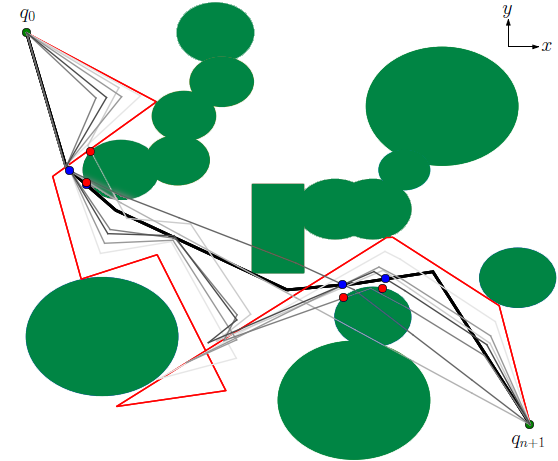
\includegraphics[width=7.5cm]{concave_final_green.png}
	\caption{Path-optimization results on a 2D-ponctual robot, moving around 
	obstacles. Initial paths are in red, optimized ones in black. Grey paths 
	represent intermediate iterations, red dots colliding configurations and blue 
	dots the associated collision-free configurations of the backtracked paths 
	where constraints have been computed.}
	\label{2D_long}
\end{figure}

Figure~\ref{2D_long} shows several iterations of our optimizer on 2D cases. Since 
in this special case, transformation constraints are equivalent to compulsory 
configurations to pass through, we can verify that our optimized path is applying 
all computed constraints. We can also understand which collisions have led to 
the constraints.

Besides, these examples give a better understanding of how the tuning of $\alpha$ 
has to balance lot of iterations and relevant collision-constraint addition. For 
example, if we alter a lot the initial path with a large gradient step and 
compute the corresponding collisions, constraints will be chosen on a very-not 
optimal path and will not be pertinent w.r.t. the obstacles we wanted to 
avoid.

Figure~\ref{2D_long} illustrates a path example that random shortcut will not manage to 
optimize in an affordable time, because of probabilistically failing to sample 
configurations in the box. Our gradient-based algorithm succeeds to optimize the 
path contained in the box, with the following cost coefficients 
$$
\lambda_{i-1} = \frac{1}{\sqrt{(\conf_{i\,0}-\conf_{i-1\,0})^T \weight^2 
(\conf_{i\,0}-\conf_{i-1\,0})}}
$$
aiming at keeping the same ratio between path segment lengths at 
minimum as at 
initial path, represented by the waypoints ($\conf_{i\,0})_{1\leq i\leq n+1}$.
Without these coefficients, the path that minimizes the cost corresponds to a 
straight line with the waypoints equidistantly allocated, which is not adapted for 
the Figure~\ref{local_box_optim} type of problems with a local passage very
constrained by obstacles. Note that this cost is also working with all other 
examples presented in this paper.


\begin{figure}[t]
	\centering
	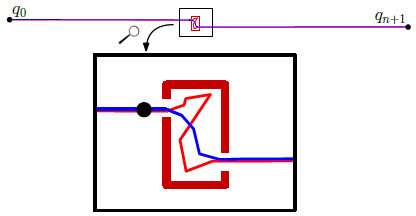
\includegraphics[width=7.5cm]{local_box_optim.png}
	\caption{Case of a long initial path (above) containing a small part that can 
	be optimized (below). Random shortcut is unlikely to optimize the part containing detours in the box, whereas our method 
	succeeds (in blue).}
	\label{local_box_optim}
\end{figure}

\begin{algorithm}
\begin{algorithmic}[1] % line numerotation
\Procedure{randomShortcut}{$\xx$}
   \State nbFailures $\gets 0$
   \While {$nbFailures < maxNbFailures$}
        \State $failure \gets true$
        \State $T \gets \mbox{upper bound of }\xx\mbox{ definition interval}$
        \State $t_1 < t_2 \gets \mbox{random numbers in }[0,T]$
        \State $lp0 \gets \texttt{steeringMethod} (\xx(0), \xx(t_1))$
        \State $lp1 \gets \texttt{steeringMethod} (\xx(t_1), \xx(t_2))$
        \State $lp2 \gets \texttt{steeringMethod} (\xx(t_2), \xx(T))$
        \State $newPath \gets \mbox{empty path defined on }[0,0]$
   	\If{$lp0$ is collision-free}
          \State $newPath \gets lp0$; $failure \gets false$
        \Else
          \State $newPath \gets \xx_{|[0,t_1]}$
        \EndIf
   	\If{$lp1$ is collision-free}
          \State $newPath \gets \texttt{concatenate} (newPath, lp1)$
          \State $failure \gets false$
        \Else
          \State $newPath \gets \texttt{concatenate} (newPath, \xx_{|[t_1,t_2]})$
        \EndIf
   	\If{$lp2$ is collision-free}
          \State $newPath \gets \texttt{concatenate} (newPath, lp2)$
          \State $failure \gets false$
        \Else
          \State $newPath \gets \texttt{concatenate} (newPath, \xx_{|[t_2,T]})$
        \EndIf
        \State $\xx \gets newPath$
        \If {$failure$} $nbFailures \gets nbFailures + 1$
        \EndIf
      \EndWhile
    \Return $\xx$
\EndProcedure
\end{algorithmic}
\caption{Random shortcut as adapted from~\cite{Sekhavat-Svestka1998} 
Section~6.4.1. \texttt{steeringMethod} returns the linear interpolation between 
two configurations. $\xx_{|I}$ denotes path $\xx$ restricted to interval $I$. 
$maxNbFailures$ is a parameter that affects time of computation and quality of 
the result.}\label{algo:random-shortcut}
\end{algorithm}

\subsection{To 3D complex problems}

We also experiment our algorithm on more complex robots, with transformation 
collision-constraints. Unless another value is given, $\alpha_{init}$ is set to 0.2.

%\begin{figure}[b]
%	\centering
%	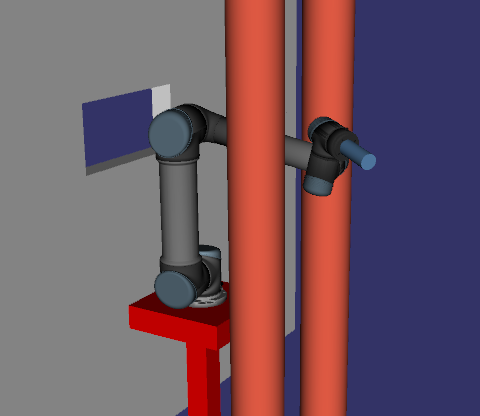
\includegraphics[width=5cm,height=3.5cm]{ur5_v2.png}
%	\caption{6-DOF robot arm on which our path-optimization has been tested.}
%	\label{ur5}
%\end{figure}


In the included video, we present four situations where our algorithm has been 
% TODO puzzle if included => 5 situations
tested and compared to random shortcut~\cite{randomShortcutHPP}
(Algorithm~\ref{algo:random-shortcut}).
The termination condition of random shortcut allows it to try 
shortening the path until 5 iterations of non-improvement are reached 
(corresponding to $maxNbFailures$ in Algorithm~\ref{algo:random-shortcut}).
%But we admit that restrincting the number of random shortcut iterations is 
%neither a acceptable criterion because of randomness.
%We also discuss the good properties and limits of our algorithm.

% analysis UR2:
On the 5-DOF double-arm problem, one arm has to get around an obstacle while the 
other is relatively far from obstacles. As expected, the initial path given by 
RRT-connect activates both arms to solve the problem. Contrary to random shortcut, 
our optimizer manages to cancel the rotation of the free-arm while optimizing the 
first arm motion. Initial path length 5.17 has been decreased to 4.55 by random shortcut and to 3.20 by the gradient-based optimizer.


% analysis UR5:
For the following example with a 6-axis manipulator arm 
%(Figure~\ref{ur5})
in a  cluttered environment, path reduction only manages to reduce some but not 
all detours. This behavior can be explained by a path over-constraining due to the 
important proximity of the robot to the obstacles during the whole path, and 
because there are not so many DOF to play on to easily avoid collisions and 
return a small-cost solution.
We advance this explanation because on the two following high-DOF examples of the video (and Figure~\ref{pr2_final}), results are better 
in terms of path length and quality.

\begin{figure}[H]
	\centering
	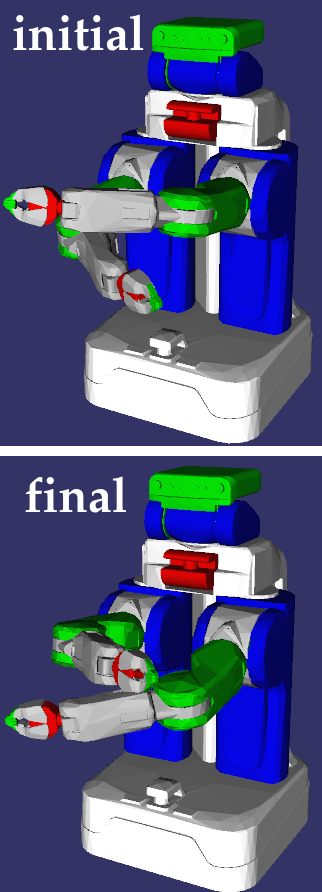
\includegraphics[height=4.9cm,width=1.8cm]{pr2_initial_final_vertical.png}
	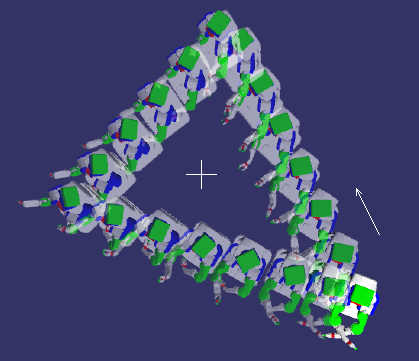
\includegraphics[width=5.7cm]{p0_pr2_alone_merged3.png}
	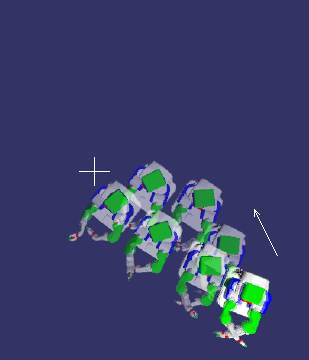
\includegraphics[height=4.9cm]{p1RS_pr2_alone_merged3.png}
	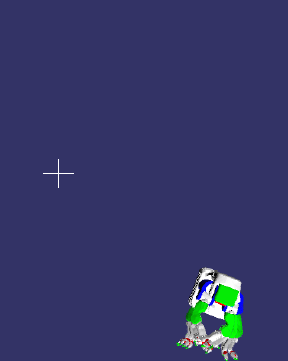
\includegraphics[height=4.9cm]{p1GB_pr2_alone_merged3.png}\\
	\caption{In this motion planning problem, PR2 robot has just to 
exchange the positions of its arms. The task is simple, however, in absence of 
explicit indication, any probabilistic motion planner will compute a path that 
makes the PR2 mobile basis purposelessly moving. This is the case of RRT-connect 
algorithm (left). Path optimization is expected to remove unnecessary motions. 
The popular random shortcut algorithm fails in this case (middle). Our algorithm 
succeeds (right).}
	\label{pr2_final}
\end{figure}

% analysis PR2 alone:
In the example presented Figure~\ref{pr2_final} and in the video, the mobile 
40-DOF PR2 simply has to cross its arms from 
the left arm up position to the right arm up one. Lengths of the initial path, the 
random shortcut optimized path and the gradient-based optimized path are 
respectively 14.5, 6.34 and 3.62. The RRT-connect planner 
returns detours and activates non-useful DOF such as the head, the torso lift 
and the translation on 
the ground. Once again, random shortcut will hardly optimize the mobile base 
translation of the robot and other unnecessary DOF uses, unlike our 
optimized-path which mainly results in moving the arms as expected 
(Figure~\ref{pr2_final} right).
%The removal 
%of the translation is also a consequence of our cost ponderation as described in 
%the previous section.
% NON ???

% analysis PR2 in kitchen:
We obtain similar results on the PR2 performing a manipulation task 
in a kitchen environment (see the video). The robot has to move 
his hands from the top to the bottom of a table.
Our optimizer manages to reduce the initial length 15.8 from the visibility-PRM 
planner and improves the path quality 
just adding transformation constraints between the table and the 
robot's arms and grippers. Thus, the robot just slightly moves 
backward and uses its arm DOF to avoid the table, instead of 
processing a large motion to get away from the table. With our method, the path length is downed to 4.59, against 8.24 for random shortcut.

Optimization computation time and path length averages are presented for 30 runs of the PR2-crossing-arms in the Table~\ref{tab:results}. In the same way, time computation averages for the PR2-in-kitchen example have been 
calculated: $59.5\,\text{s}$ (gradient-based optimizer) and $76.2\,\text{s}$ (random shortcut).
Thus our method presents 
similar computation times and path lengths for mobile manipulation tasks. However, the extinction of the mobile base motion in the gradient-based optimized path is advanced in the right column of Table~\ref{tab:results}. Thus the problem addressed 
Figure~\ref{decoupled_DOF_optimization} is solved considering this DOF.


\begin{table}[t]
\centering
  \begin{tabular}{cccc}
  \\
  \toprule
     & Computation & Path  & Traveled distance\\
     & time & length & by the base\\
    \midrule
    \midrule
    Initial &  & $13.7$ & $10.9$\\
    Gradient-based & $\,781\text{ms}$ & $3.69$ & $10^{-6}$\\
    Random shortcut & $\,823\text{ms}$ & $3.82$ & $2.94$\\
    \bottomrule
  \end{tabular}
\caption {Results for 30 runs of the PR2-crossing-arms example. For each run, a solution path is planned by Visibility-PRM as initial guess for each optimizer. $\alpha_{init}$ is set to 0.2. The right column represents the distance that is traveled by the robot mobile base during the path.}
\label{tab:results}
\end{table}

\section{CONCLUSIONS}
We managed to settle a path optimization for decoupled-DOF robots such as mobile 
manipulators. Our algorithm uses standard numerical tools as collision checking 
and QP resolution, and correlates them in a 
simple but effective way, playing on the scalar iteration parameter. Therefore, 
our method only require few distances computation, so geometry pre-processing or 
offline optimization are not necessary to remain time competitive. We demonstrate 
that the optimizer is 
time-competitive comparing to random shortcut and proposes better quality paths 
for high-DOF robots, removing unnecessary DOF motions. Our optimizer also manages 
to reduce a local detour in a long path while random shortcut methods will mostly 
fail.

The experimental results show that transformation constraints may in some cases be overconstraining. We also tried distance constraints without much success due to the non-continuous differentiability of distance. In a future work, we will study other one-dimensional constraints in order to achieve better results.

\bibliographystyle{tADR} % plain, alpha, abbr, unsrt
\bibliography{paper}

\end{document}
